\documentclass[11pt, oneside]{article}   	% use "amsart" instead of "article" for AMSLaTeX format


% \usepackage{draftwatermark}
% \SetWatermarkText{Draft}
% \SetWatermarkScale{5}
% \SetWatermarkLightness {0.9} 
% \SetWatermarkColor[rgb]{0.7,0,0}

%
%	TikZ
%
\usepackage{tikz}
\usetikzlibrary{angles, quotes}
\usetikzlibrary{calc}
\usetikzlibrary{intersections}
\usetikzlibrary{arrows,backgrounds,calc,patterns,angles,quotes,shapes,calc,decorations,through,lindenmayersystems}    
\usepackage{tkz-euclide}
\usepackage{pgfplots}
%
%
%
\usepackage{geometry}                		% See geometry.pdf to learn the layout options
\geometry{letterpaper}                   		% ... or a4paper or a5paper or ... 
%\geometry{landscape}                		% Activate for for rotated page geometry
%\usepackage[parfill]{parskip}    		% Activate to begin paragraphs with an empty line rather than an indent
\usepackage{graphicx}				% Use pdf, png, jpg, or eps� with pdflatex; use eps in DVI mode
								% TeX will automatically convert eps --> pdf in pdflat						
								% TeX will automatically convert eps --> pdf in pdflatex		
\usepackage{amssymb}
\usepackage{mathrsfs}
\usepackage{hyperref}
\usepackage{url}
\usepackage{subcaption}
\usepackage{authblk}
\usepackage{amsmath}
\usepackage{mathtools}
\usepackage{graphicx}
\usepackage[export]{adjustbox}
\usepackage{hyperref}
\usepackage{alltt}
\usepackage{color}
\usepackage[utf8]{inputenc}
\usepackage[english]{babel}
\usepackage{float}
\usepackage{bigints}
\usepackage{braket}
\usepackage{siunitx}
\usepackage{relsize}


%
% compatability
%
\pgfplotsset{compat=1.17} 

\begin{document}

%
% bloch sphere
%
\bigskip
\begin{figure}[H]
\centering
  \resizebox{0.70 \textwidth}{!} {	
  
  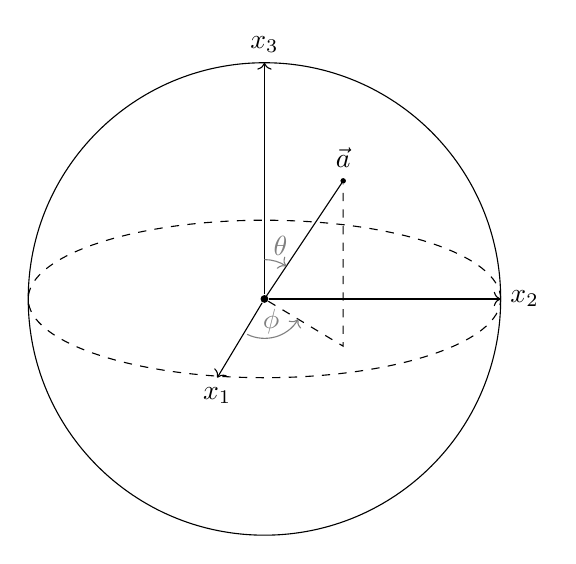
\begin{tikzpicture}

  % Define radius
  \def\r{3}

  % Bloch vector
  \draw (0, 0) node[circle, fill, inner sep=1] (orig) {} -- (\r/3, \r/2) node[circle, fill, inner sep=0.7, label=above:$\vec{a}$] (a) {};
  \draw[dashed] (orig) -- (\r/3, -\r/5) node (phi) {} -- (a);

  % Sphere
  \draw (orig) circle (\r);
  \draw[dashed] (orig) ellipse (\r{} and \r/3);

  % Axes
  \draw[->] (orig) -- ++(-\r/5, -\r/3) node[below] (x1) {$x_1$};
  \draw[->] (orig) -- ++(\r, 0) node[right] (x2) {$x_2$};
  \draw[->] (orig) -- ++(0, \r) node[above] (x3) {$x_3$};

  % Angles
  \pic [draw=gray, text=gray, ->, "$\phi$"] {angle = x1--orig--phi};
  \pic [draw=gray, text=gray, <-, "$\theta$", angle eccentricity=1.4] {angle = a--orig--x3};

\end{tikzpicture}
     
  }																					 								% end resizebox                                                            
 \caption{The Bloch Sphere}
 \label{fig:bloch_sphere}
\end{figure}
																						% resize figure if you want



%
%	draw Pythagorean theorem stuff
%
\bigskip
\begin{figure}[H]
\centering
  \resizebox{0.70 \textwidth}{!} {																							% resize figure if you want
  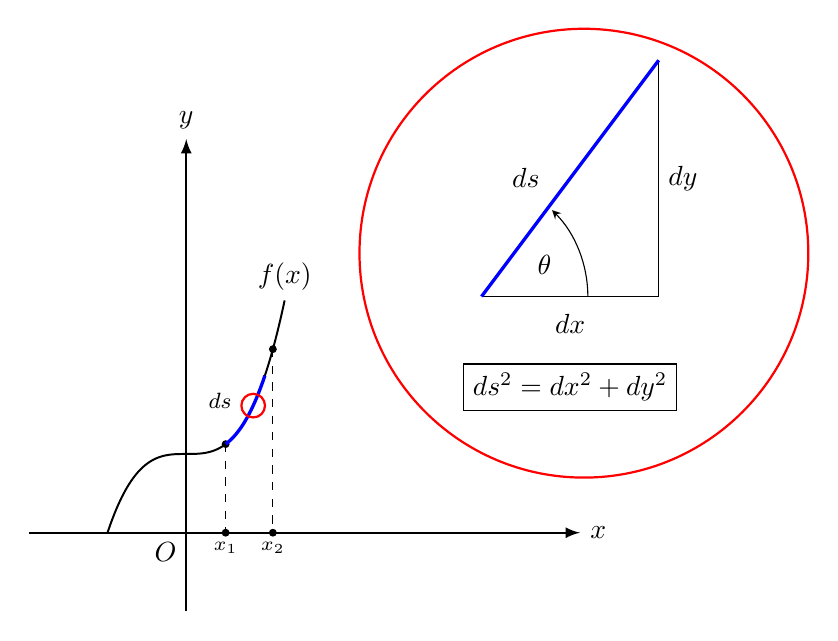
\begin{tikzpicture} [every edge quotes/.append style = {anchor=south, sloped}, declare function={f(\x)=1 + \x*\x*\x;}]	% define f(x)
       \draw[thick, -latex] (-2,0) -- (5,0) coordinate [label={[right] $x$}];  												% x axis
       \draw[thick, -latex] (0,-1) -- (0,5) coordinate [label={[above] $y$}]; 												% y axis
       \draw [line width=0.25mm, smooth, samples=100,domain=-1.0:1.25] plot (\x,{f(\x)});									% draw f(x)
       \draw [draw=none] (1.25, {f(1.25)}) coordinate [label={[above] $f(x)$}];												% label f(x)
       \coordinate (O) at (0,0); 
       \path (O) node[below left] {$O$};  
%
%	various coordinates
%     
       \coordinate (x1y1) at (0.5,{f(0.5)});
       \coordinate (x1y0) at (0.5,0.0);
       \coordinate (x2y2) at (1.1,{f(1.1});
       \coordinate (x2y0) at (1.1,0.0);
       \coordinate (cir) at (0.85,{f(0.85)});
%
       \fill (x1y1) circle (0.05);																					% put a dot on the curve at x1y1
       \fill (x2y2) circle (0.05);																					% put a dot on the curve at x2y2
	   \draw [very thick,blue,smooth,samples=100,domain=0.5:1.0] plot (\x,{f(\x)});									% draw blue segment on f(x)
       \draw[draw=none] (x1y1) -- (x2y2) coordinate [label={[font=\footnotesize, yshift=-0.05cm, xshift=-0.10cm, midway,left] \color{black} $ds$}];
       \draw[dashed] (x1y1) -- (x1y0) coordinate [label={[font=\scriptsize,below] \color{black} $x_1$}];
       \draw[dashed] (x2y2) -- (x2y0) coordinate [label={[font=\scriptsize,below] \color{black} $x_2$}];
       \fill (x1y0) circle (0.05);																					% put a dot on the x axis at x1
       \fill (x2y0) circle (0.05);																					% put a dot on the x axis at x2
       \draw[red, thick] (cir) circle (0.150);																		% put a circle on f(x) where ds is
       

     
%
%	draw triangle and circle to show ds
%   
%
%
%	set up triangle coordinates
%
	   \coordinate (a) at (3.75,3.00);
	   \coordinate (c) at (6.00,3.00);
	   \coordinate (b) at (6.00,6.00);
%
%	draw the triangle
%	   
       \draw[] (a) -- (c) coordinate [label={[yshift=-0.1cm,midway,below] ${dx}$}];										% dx
       \draw[] (c) -- (b) coordinate [label={[midway,right] ${dy}$}];													% dy
       \draw[blue,very thick] (a) -- (b) coordinate [label={[xshift=-0.25cm,midway,left] \color{black} ${ds}$}];		% ds
       \draw[draw=none]  (a) -- (c) node[draw,rectangle,yshift=-0.85cm,midway,below] {${ds^2 = dx^2 + dy^2}$};			% draw the pythagorean theorem
       \draw[red,thick] (5.05,3.55) circle (2.85);																		% big circle
%
%	draw the angle      
%       
       \node[xshift=-2mm, yshift=-2mm] at (4.75,3.60) {$\theta$};
       \draw[-stealth,thin] (5.10,3.00) arc (0:45:1.55cm);
%
%	done
%
     \end{tikzpicture}
    }																					 								% end resizebox                                                            
 \caption{$f(x)$, $ds$ and the Pythagorean Theorem}
 \label{fig:pythagorean_theorem}
\end{figure}



%
% old
%
%
%	draw Pythagorean theorem stuff
%
\bigskip
\begin{figure}[H]
\centering
  \resizebox{0.70 \textwidth}{!} {																							% resize figure if you want
  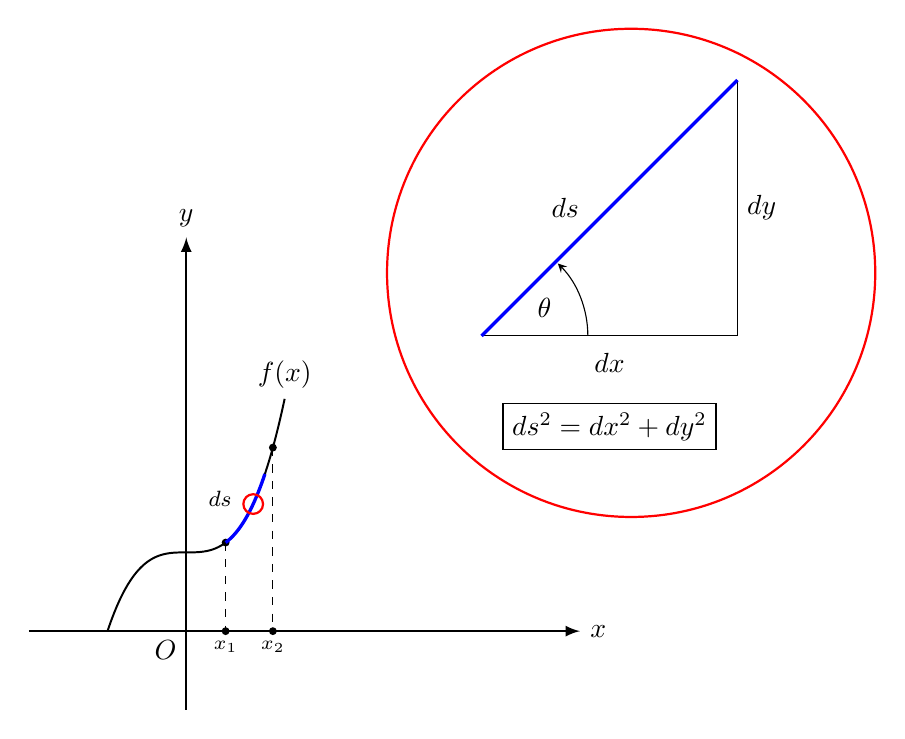
\begin{tikzpicture} [every edge quotes/.append style = {anchor=south, sloped}, declare function={f(\x)=1 + \x*\x*\x;}]	% define f(x)
       \draw[thick, -latex] (-2,0) -- (5,0) coordinate [label={[right] $x$}];  												% x axis
       \draw[thick, -latex] (0,-1) -- (0,5) coordinate [label={[above] $y$}]; 												% y axis
       \draw [line width=0.25mm, smooth, samples=100,domain=-1.0:1.25] plot (\x,{f(\x)});									% draw f(x)
       \draw [draw=none] (1.25, {f(1.25)}) coordinate [label={[above] $f(x)$}];												% label f(x)
       \coordinate (O) at (0,0); 
       \path (O) node[below left] {$O$};  
%
%	various coordinates
%     
       \coordinate (x1y1) at (0.5,{f(0.5)});
       \coordinate (x1y0) at (0.5,0.0);
       \coordinate (x2y2) at (1.1,{f(1.1});
       \coordinate (x2y0) at (1.1,0.0);
       \coordinate (cir) at (0.85,{f(0.85)});
%
       \fill (x1y1) circle (0.05);																					% put a dot on the curve at x1y1
       \fill (x2y2) circle (0.05);																					% put a dot on the curve at x2y2
	   \draw [very thick,blue,smooth,samples=100,domain=0.5:1.0] plot (\x,{f(\x)});									% draw blue segment on f(x)
       \draw[draw=none] (x1y1) -- (x2y2) coordinate [label={[font=\footnotesize, yshift=-0.05cm, xshift=-0.10cm, midway,left] \color{black} $ds$}];
       \draw[dashed] (x1y1) -- (x1y0) coordinate [label={[font=\scriptsize,below] \color{black} $x_1$}];
       \draw[dashed] (x2y2) -- (x2y0) coordinate [label={[font=\scriptsize,below] \color{black} $x_2$}];
       \fill (x1y0) circle (0.05);																					% put a dot on the x axis at x1
       \fill (x2y0) circle (0.05);																					% put a dot on the x axis at x2
       \draw[red, thick] (cir) circle (0.125);																		% put a circle on f(x) where ds is
     
%
%	draw triangle and circle to show ds
%   
%
%
%	set up triangle coordinates
%
	   \coordinate (a) at (3.75,3.75);
	   \coordinate (c) at (7.00,3.75);
	   \coordinate (b) at (7.00,7.00);
%
%	draw the triangle
%	   
       \draw[] (a) -- (c) coordinate [label={[yshift=-0.1cm,midway,below] ${dx}$}];										% dx
       \draw[] (c) -- (b) coordinate [label={[midway,right] ${dy}$}];													% dy
       \draw[blue,very thick] (a) -- (b) coordinate [label={[xshift=-0.25cm,midway,left] \color{black} ${ds}$}];				% ds
       \draw[draw=none]  (a) -- (c) node[draw,rectangle,yshift=-0.85cm,midway,below] {${ds^2 = dx^2 + dy^2}$};			% draw the pythagorean theorem
       \draw[red,thick] (5.65,4.55) circle (3.10);																		% big circle
%
%	draw the angle      
%       
       \node[xshift=-2mm, yshift=-2mm] at (4.75,4.30) {$\theta$};
       \draw[-stealth,thin] (5.10,3.75) arc (0:45:1.30cm);
%
%	done
%
     \end{tikzpicture}
    }																					 								% end resizebox                                                            
 \caption{$f(x)$, $ds$ and the Pythagorean Theorem}
 \label{fig:pythagorean_theorem}
\end{figure}




\end{document}
